\documentclass{article}
\usepackage[utf8]{inputenc}
\usepackage{latexsym}
\usepackage{amsfonts}
\usepackage{graphicx}
\usepackage{color}
\usepackage{amsthm}
\usepackage{amsmath}
\usepackage{amssymb}
\usepackage[arrow,matrix,curve,cmtip,ps]{xy}
\usepackage{verbatim}
\setlength{\parindent}{0in}
\setlength{\oddsidemargin}{0in}
\setlength{\textwidth}{6.5in}
\setlength{\textheight}{8.8in}
\setlength{\topmargin}{0in}
\setlength{\headheight}{18pt}

\usepackage{graphicx}
\graphicspath{ {Ex. 1.jpg} }

\title{TMATH 450:  Mathematics Capstone}
\author{Hannah Price and Rain Wilson}
\date{June 2020}

\begin{document}

\maketitle

\section*{Hannah's Example Problem:}\\
This is my example problem of turning a rectangle into a square. The top is a more general representation of my understanding, please correct me if I am wrong. The bottom left is a specific example where a 16 by 4 rectangle is turned into an 8 by 8 square.\\

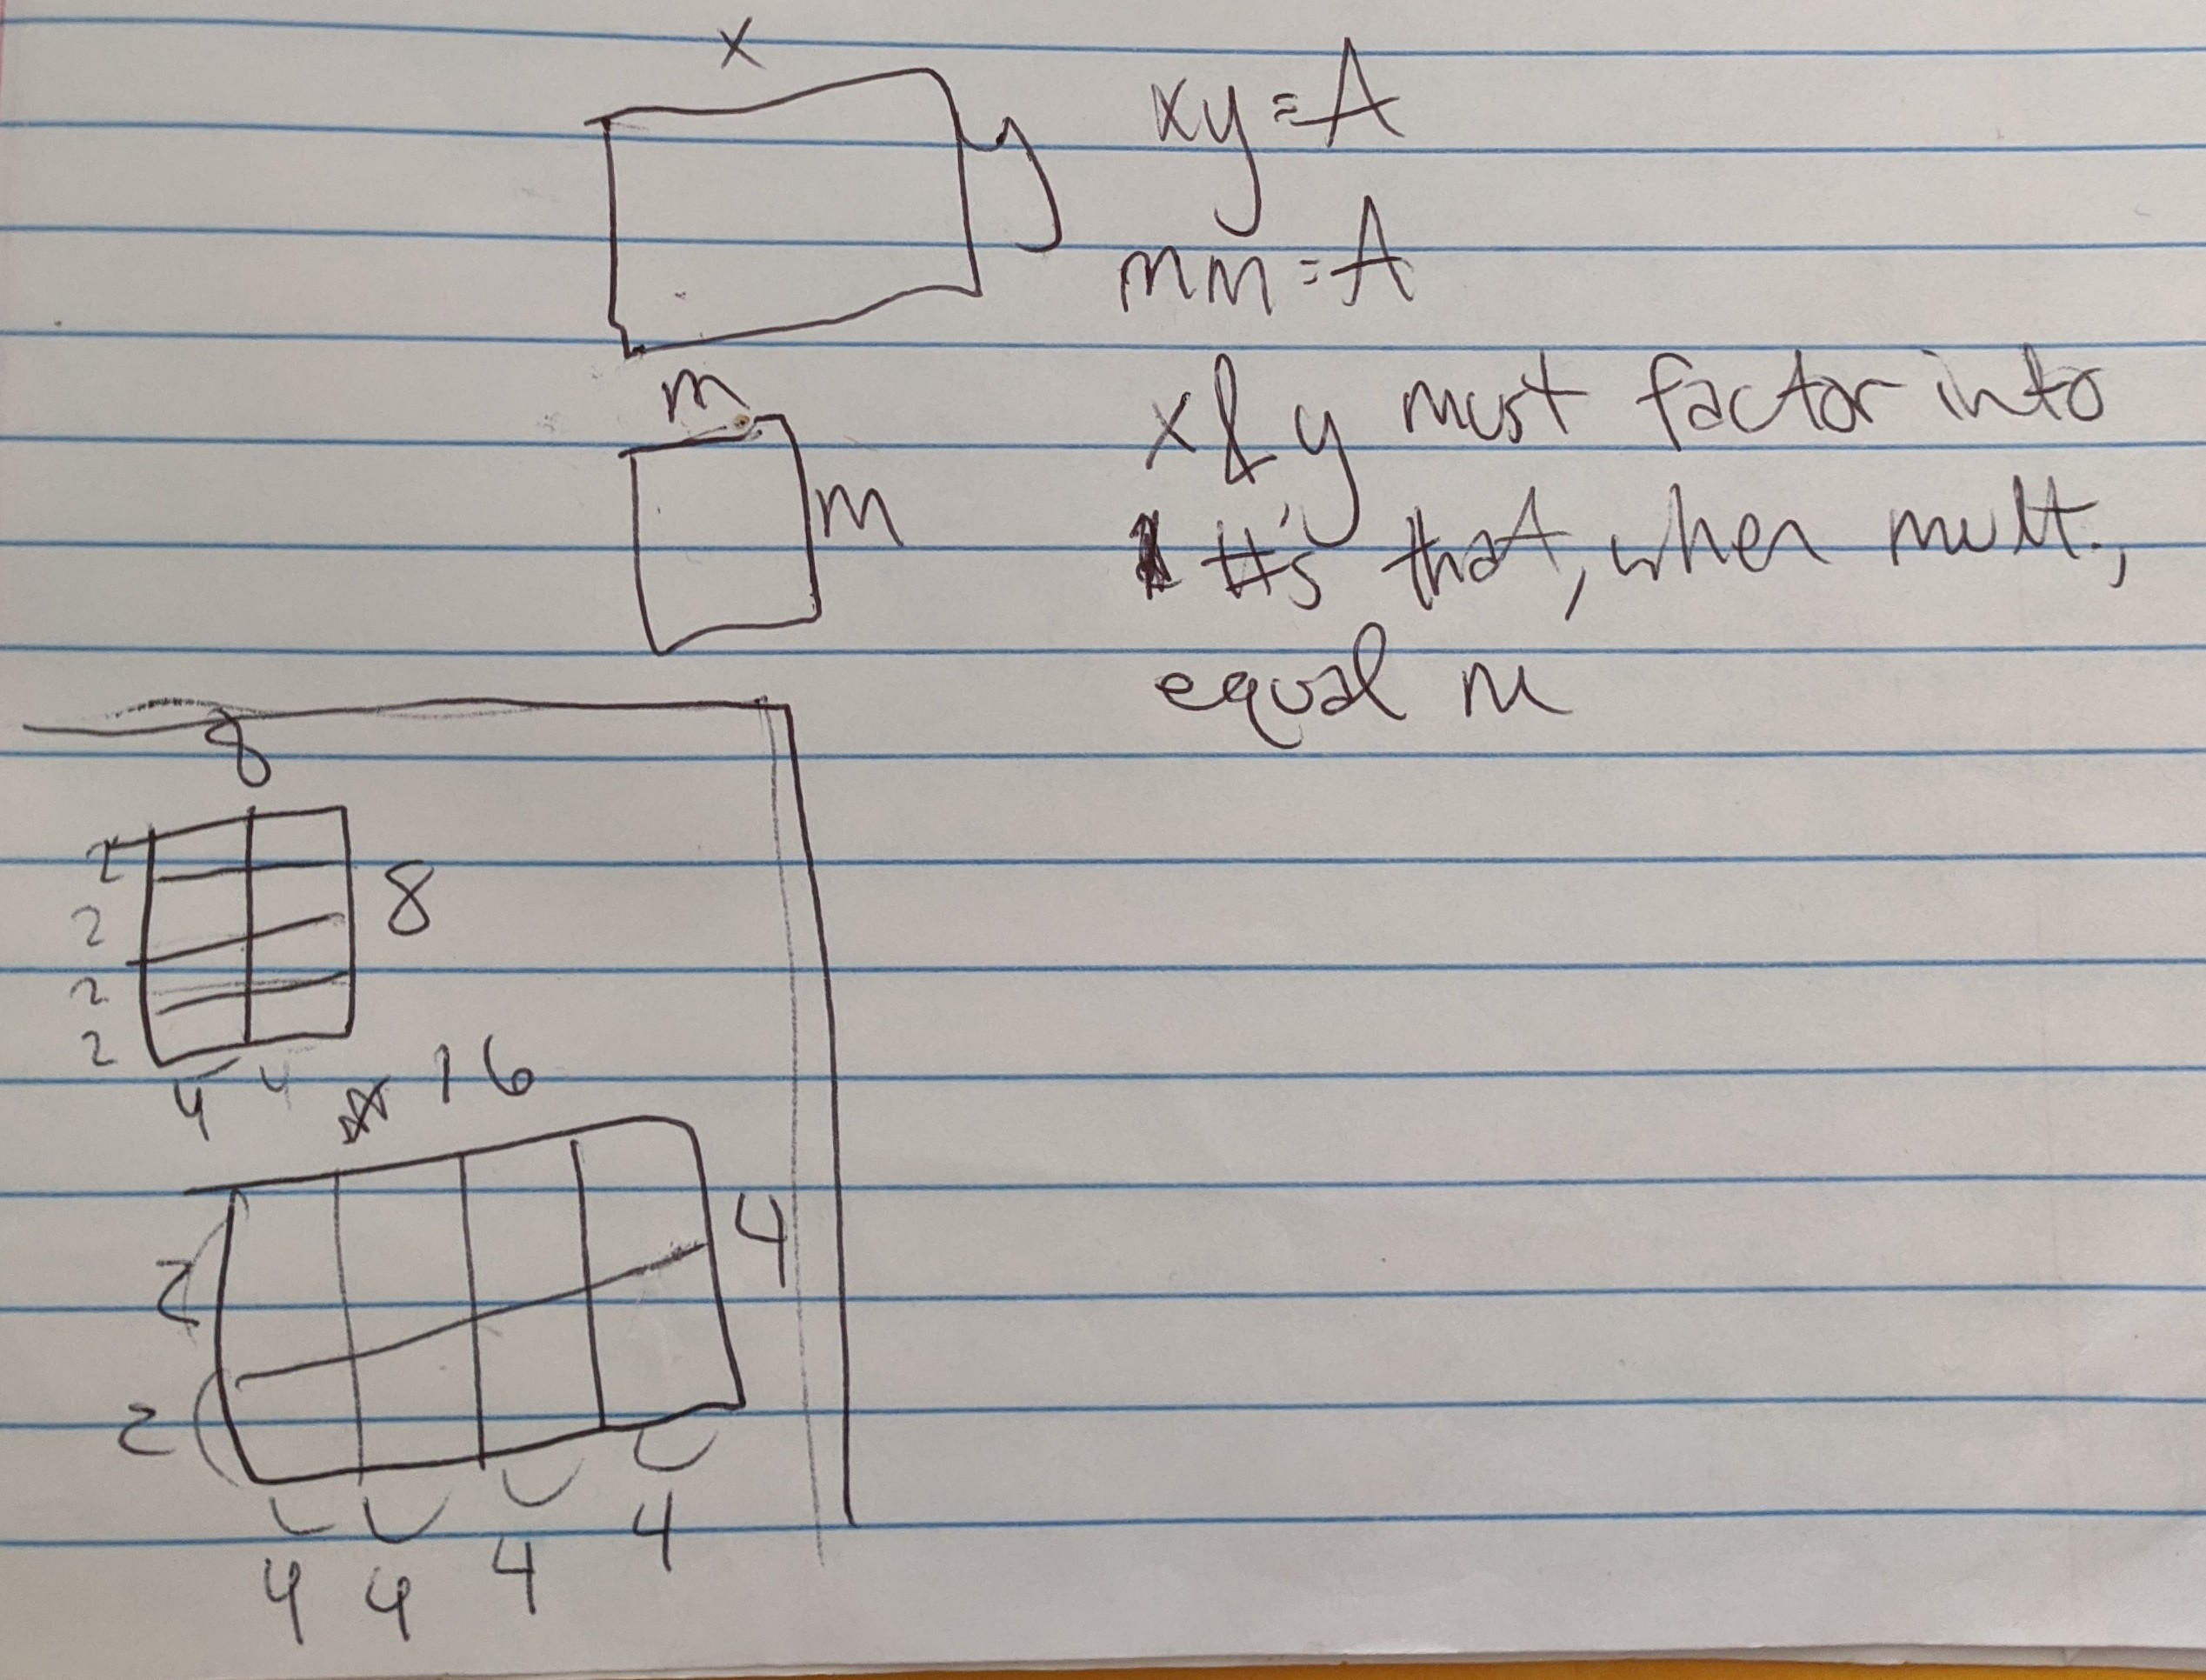
\includegraphics[width=10cm]{Ex. 1.jpg}\\

\section*{Hannah's Revised Example Problem:}\\
After reviewing the feedback on my previous example, here is a revised version. I tried to do an example for turning a 1 by 2 unit rectangle into a square. I had a particularly difficult time with this. I tried cutting it up different ways for a long time and could never seem to get it just right. After watching the recording, I looked closely at Figure 2.1.10 (Part 2). Is that what I am supposed to be doing here? I was confused because it was going from square to rectangle instead of the other way around.\\
As for my old problem with the 16 by 4 rectangle and 8 by 8 square, here is an edit of that.\\
Here, we are starting off with a 16 by 4 unit rectangle. It is separated (as shown in the picture above) into eight 2 by 4 smaller rectangles. We want to adjust these to create an 8 by 8 square. We know it is 8 by 8 because that will result in the same area (64 units squared) as the rectangle.\\

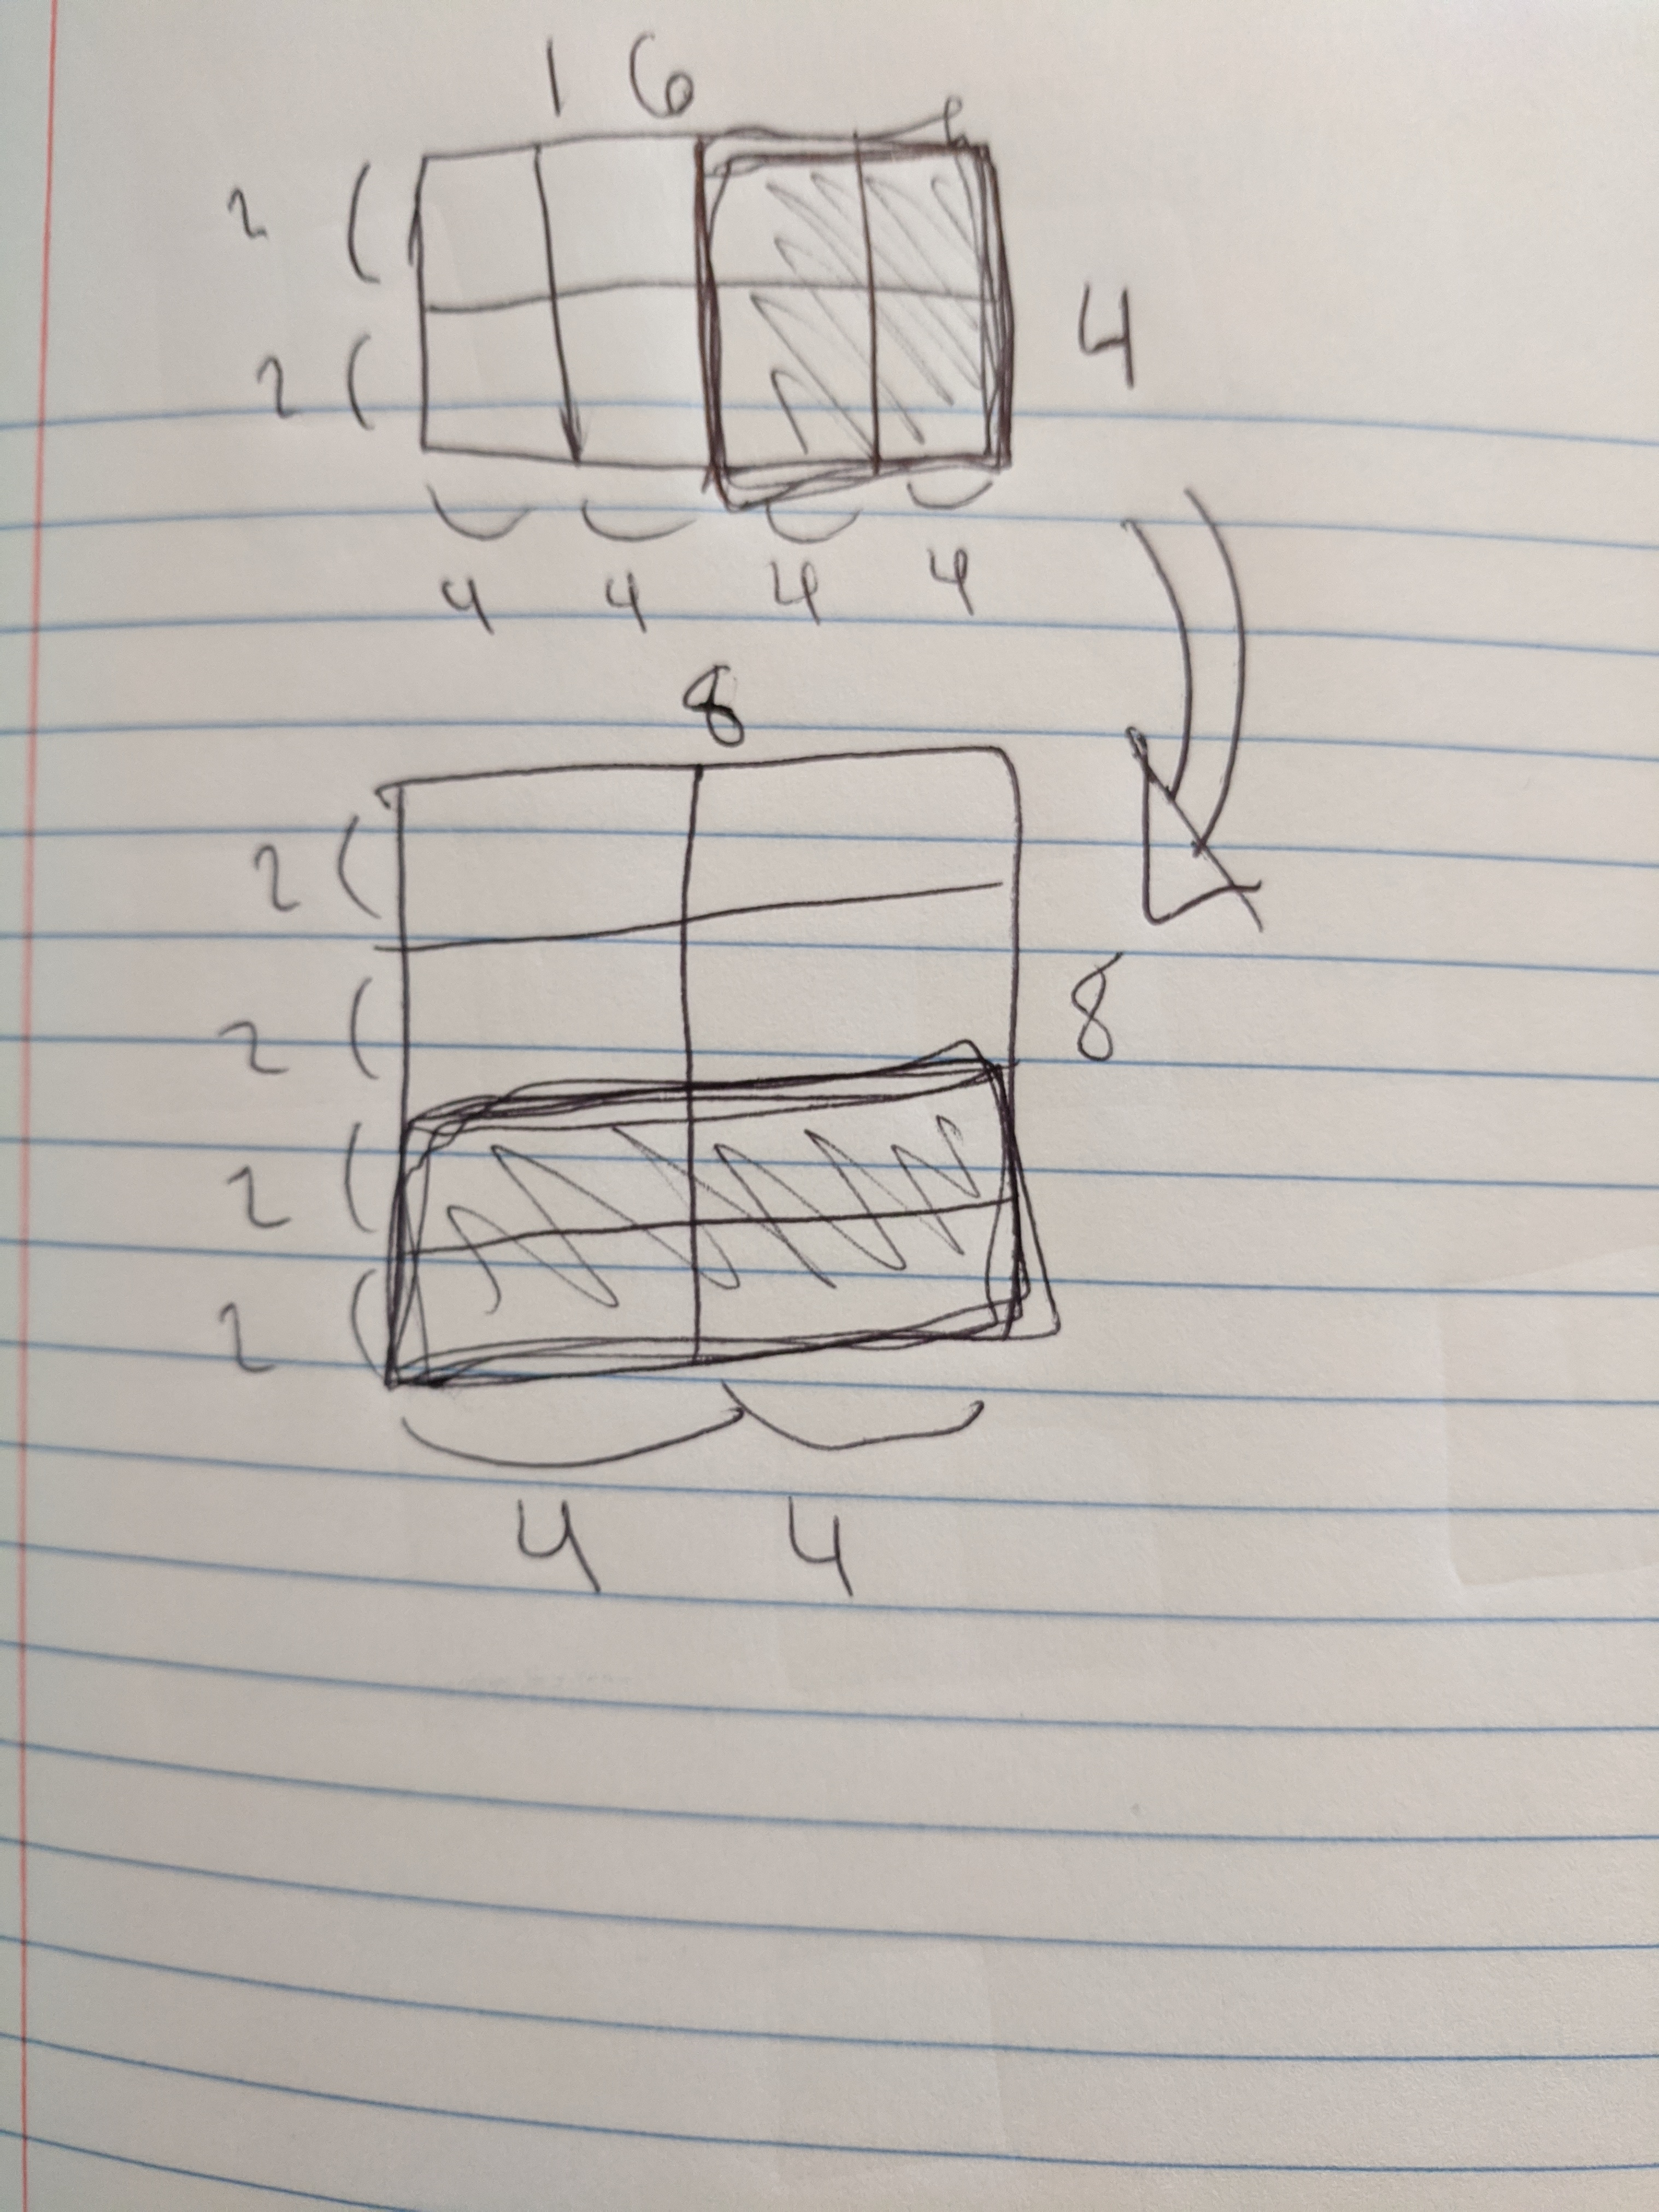
\includegraphics[width=10cm]{Ex 2.jpg}\\

While this drawing is not proportionally accurate, it shows how it is cut up and rearranged. Four of the smaller rectangles are moved to the bottom and turns it into an 8 by 8 square. We know this is a square because, as shown by the labeling, each side is 8 units across. All four side lengths being equal is a square in this case. \\

I will be happy to be this specific on the 1 by 2 unit rectangle, I am currently unsure how to do that however. I spent a decent while on it, but couldn't figure it out!\\

\section*{Hannah's Next Example Problem:}
I wasted many sheets of paper and some low-grade digital art trying to figure out Ryan's suggestion. I'll get it one day, but it is losing me a little even after viewing the recording. I was unsure where to go after following the next several steps after 3.2.5. When it came to Ruth's suggestion, I didn't get very far because I felt it was too similar to my previous example, and I was unsure of where to go as well because it didn't work last time I attempted that method. After trying all three suggestions, I got the furthest with Rain's suggestion of using three triangles.
This is where I would like some help.

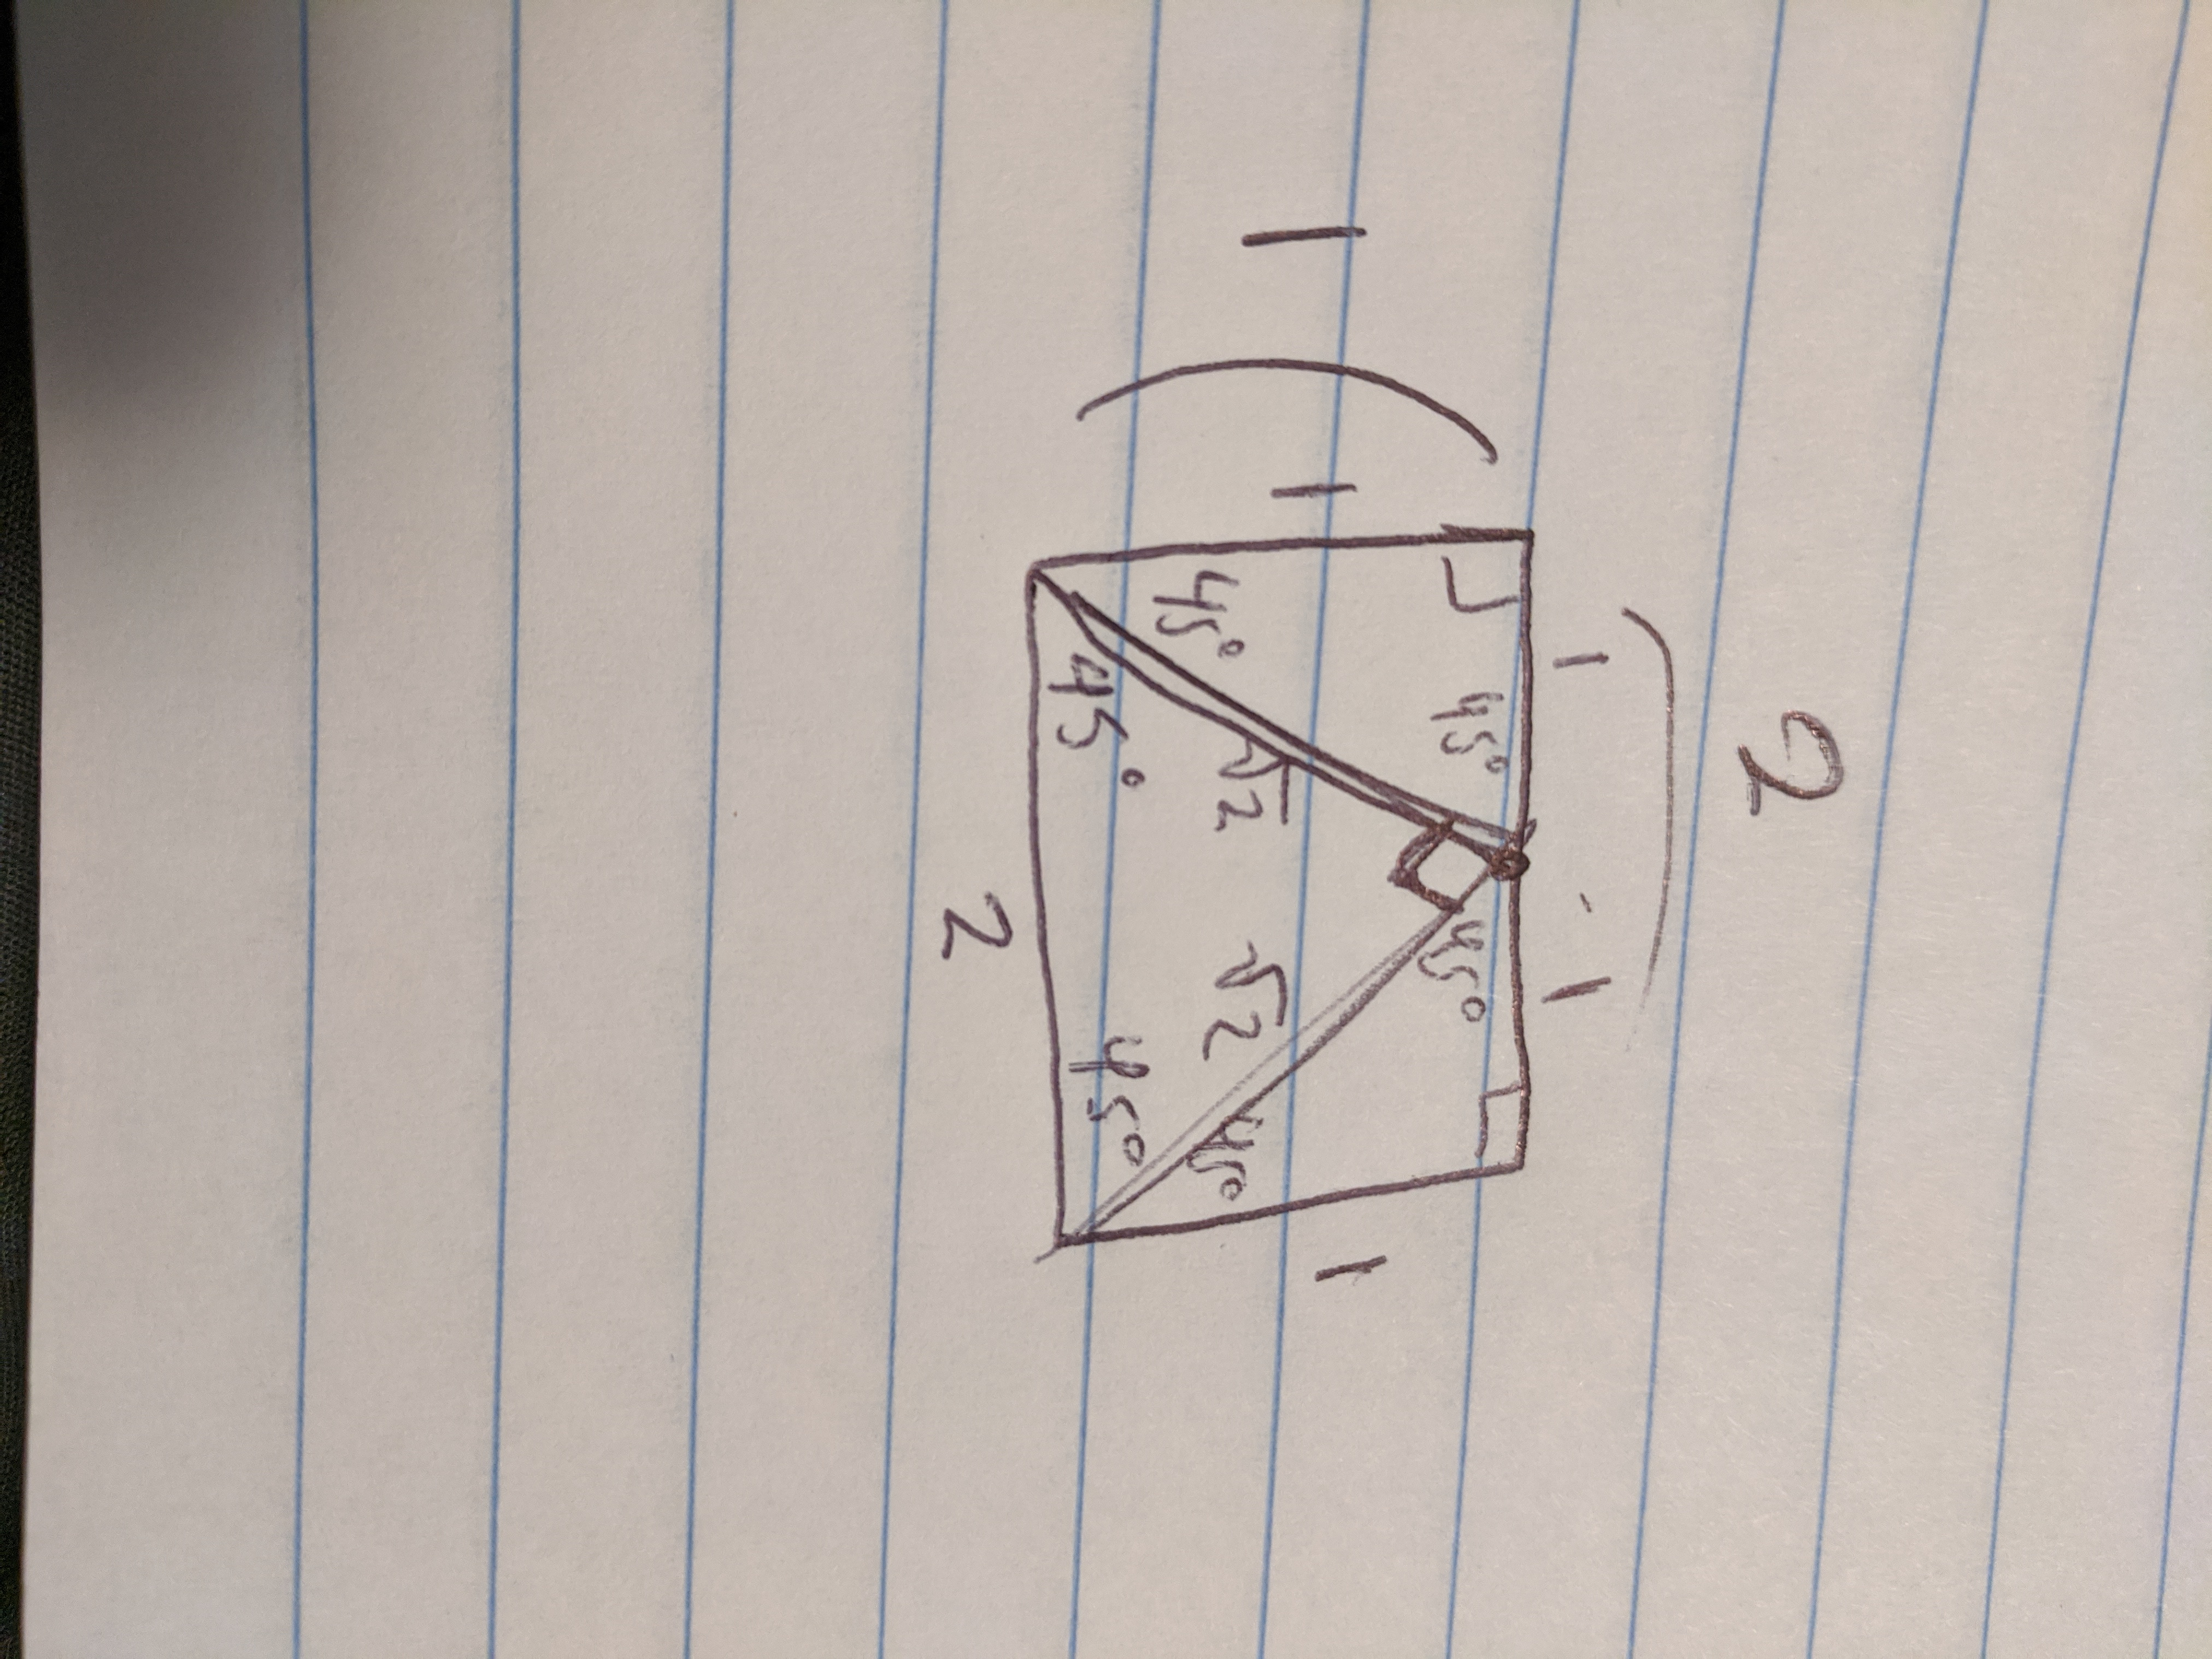
\includegraphics[width=12cm]{Ex 4.jpg}\\
\caption{Figure 1: The 2 by 1 rectangle cut into 3 triangles (skewed camera angle)}\\

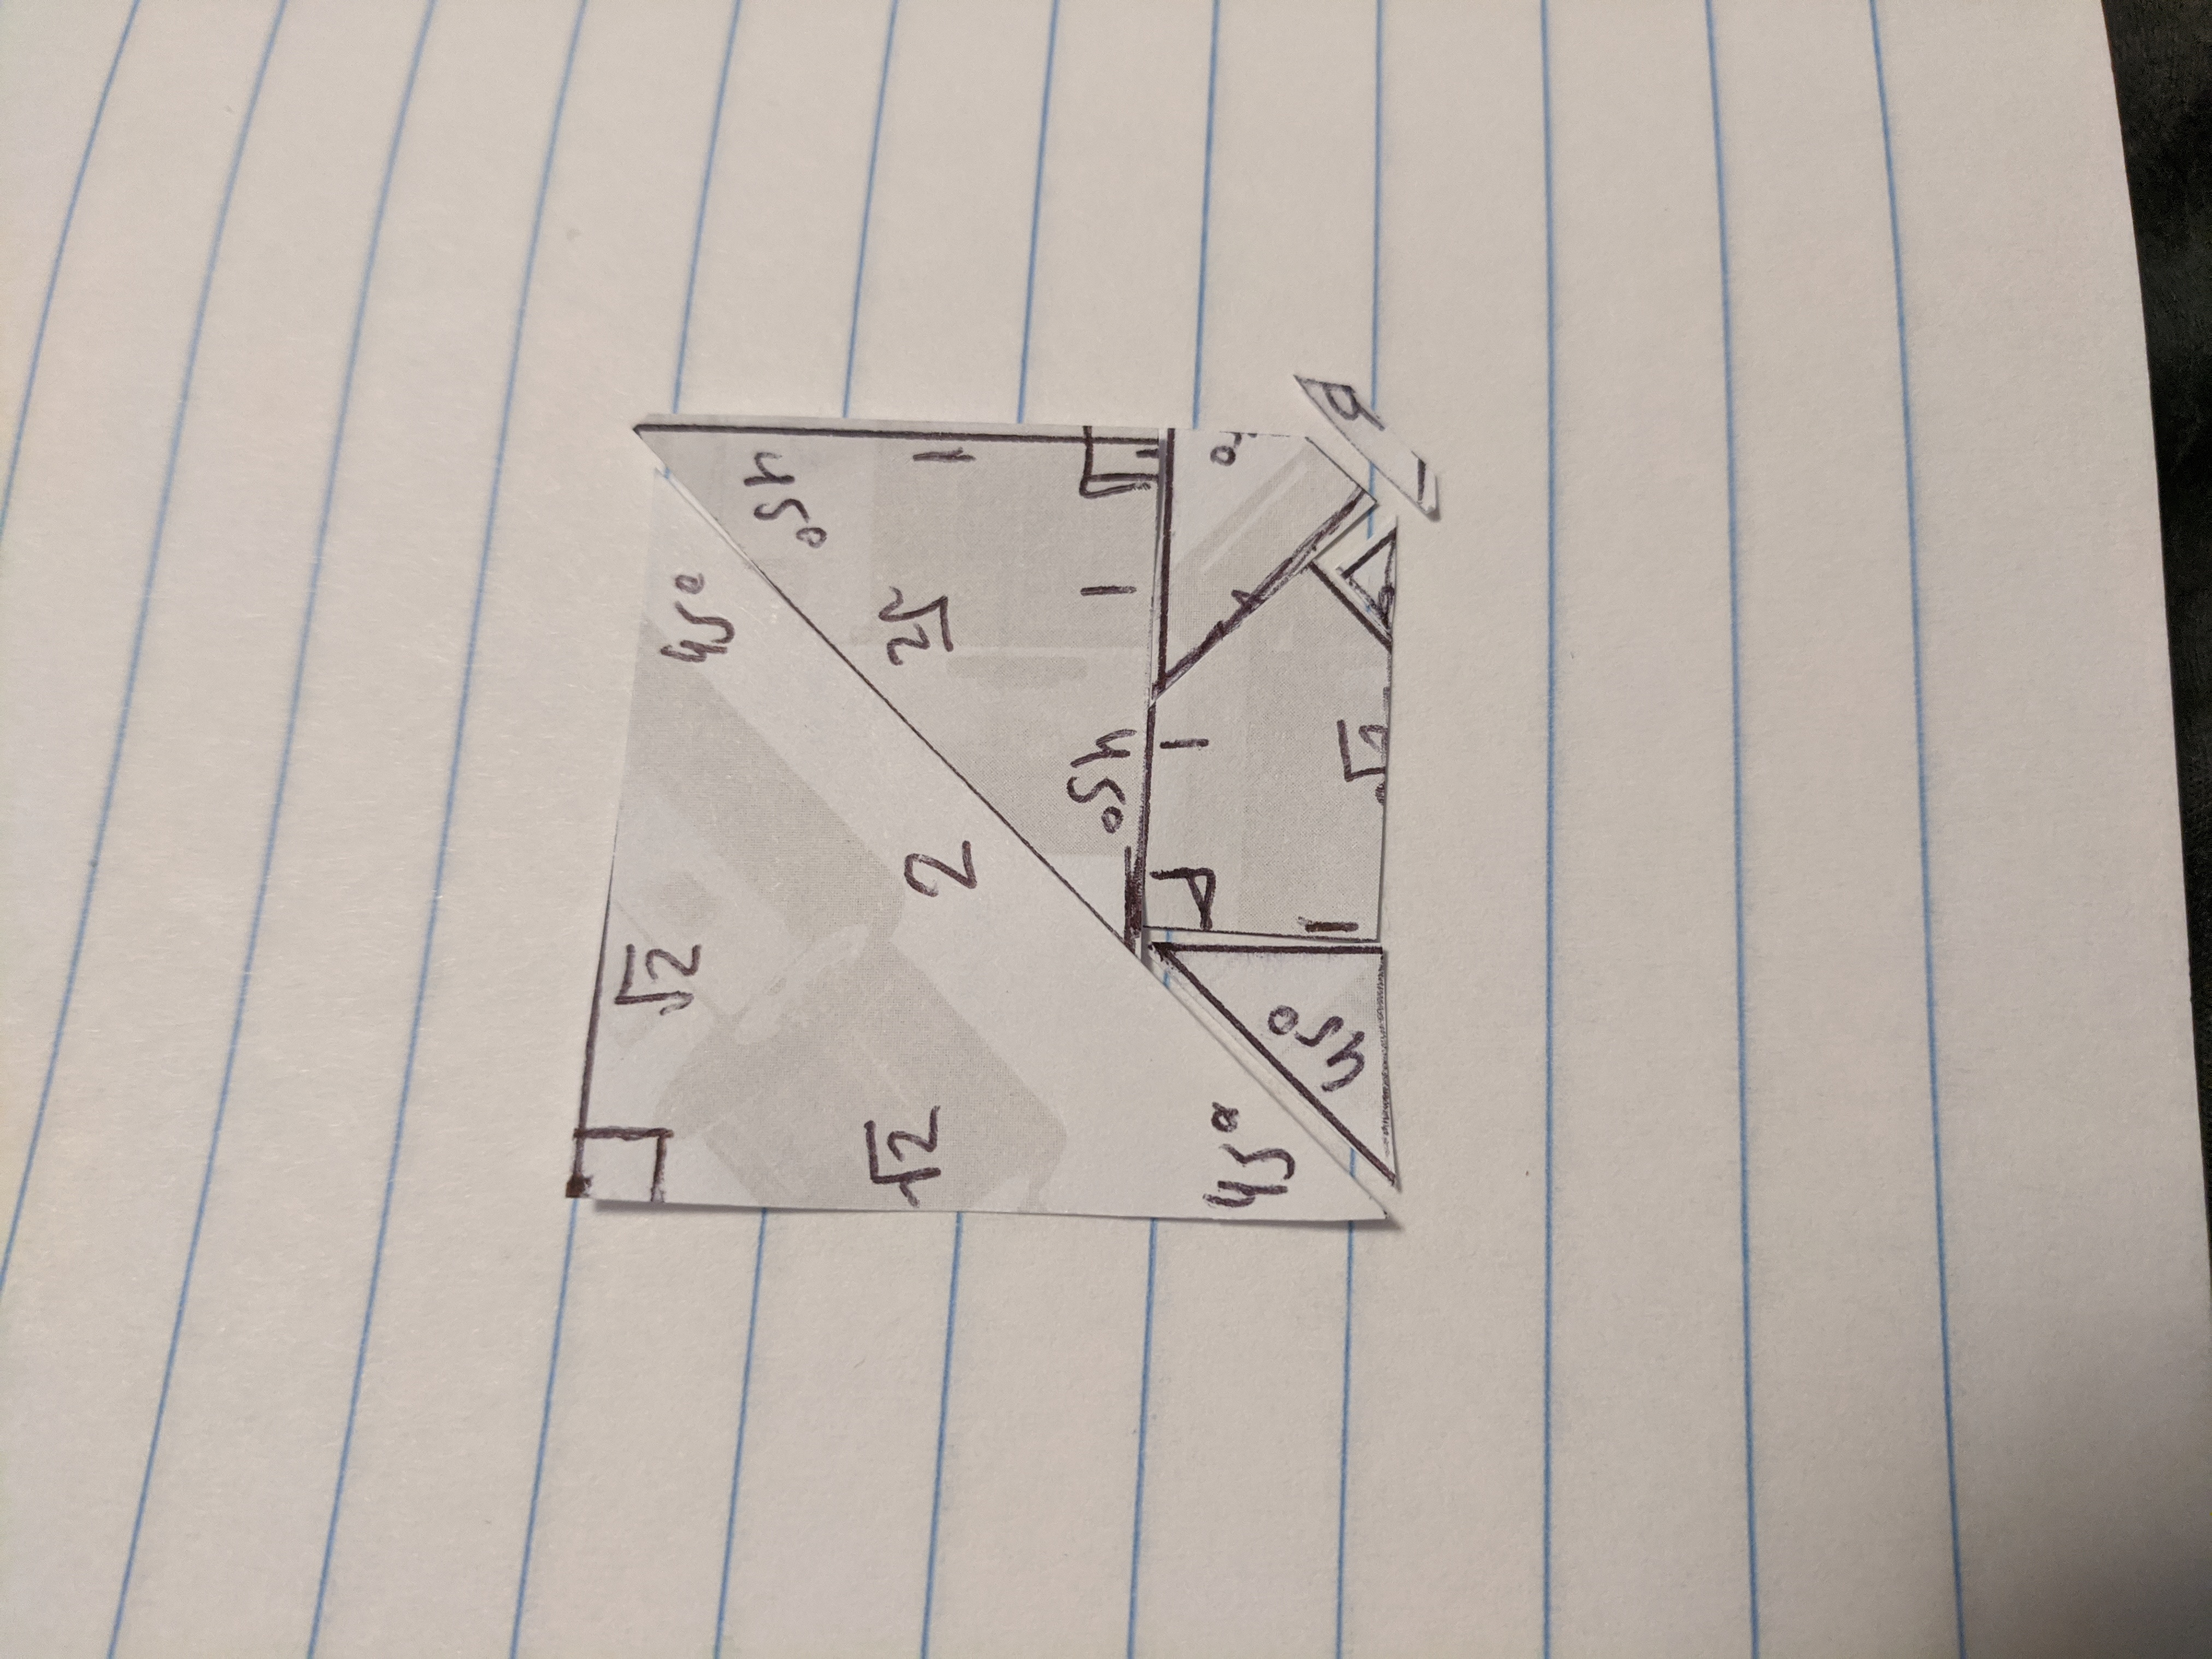
\includegraphics[width=12cm]{Ex 3.jpg}\\
\caption{Figure 2: The 3 triangles positioned and cut into an almost square (skewed camera angle)}\\

Figure 1 shows the 2 by 1 rectangle that I was trying to turn into a $\sqrt{2}$ by $\sqrt{2}$ square. By making a point in the center of a side of 2 length, I was able to create two classic 45-45-90 triangles and one $\sqrt{2}$-$\sqrt{2}$-2 triangle. This is where it started to look promising.\\
I started to piece the parts together, using the large triangle as a corner because of the 90-degree angle and building the other two around it. I cut up one of the smaller triangles as I saw fit.\\
However, I ran into a problem. As seen in Figure 2, that last little bit in the bottom right corner didn't fit. The writing/labeling of numbers may also look odd, but it was mostly for my own sake when I was arranging them. The view of them changed when I started to cut up that smaller triangle. The picture is a little skewed (I took it at an angle to avoid a shadow), but trust me when I saw that it was a square when viewed in person. It seems that I had miscalculated somewhere because there was a little bit of extra area.\\
The question I had is, could that be human error since none of my cuts could have been perfect? If it was purely theoretical, could that last little bit fit? I want to know if I did it correctly, if there was paper error, or if I need to keep searching for a way.\\
I hope this is everything you all were asking of me. Please let me know if I need to elaborate more or if I missed something that I was supposed to do!

\section*{Hannah's Next Assignment:}\\
- To clarify because of a question I have received, I had gotten lost trying to complete a process such as the one shown in diagram 3.2.5 on page 75. The steps shown in that section, (1) - (6), were what I was trying to achieve. I then wondered if going to page 76 was even what I needed to do in order to complete the question at hand which was to turn a 1 by 2 unit rectangle into a square.\\

- I decided to start by creating the square as my starting polygon and using the steps outlines in 3.2 to create the rectangle. Once I have that done, I would work backwards to see the steps that I need to take to do it in the correct order. I divided the square into two triangles by making a diagonal cut between two opposite corners. I then cut those two equal triangles to create two equal rectangles such as Figure 3.2.3 in the text.\\
Each triangle has side lengths of $\sqrt{2}$, $\sqrt{2}$, and 2 units. Using geometry, I have determined that the final rectangle will be 2 units wide and .5 units tall. I used general given rules in basic geometry to determine this by the Pythagorean Theorem, angle rules, and similar/basic techniques. \\
Also, please excuse the truck company paper, haha. The notepad it is in is very helpful.\\
Substep 1:\\
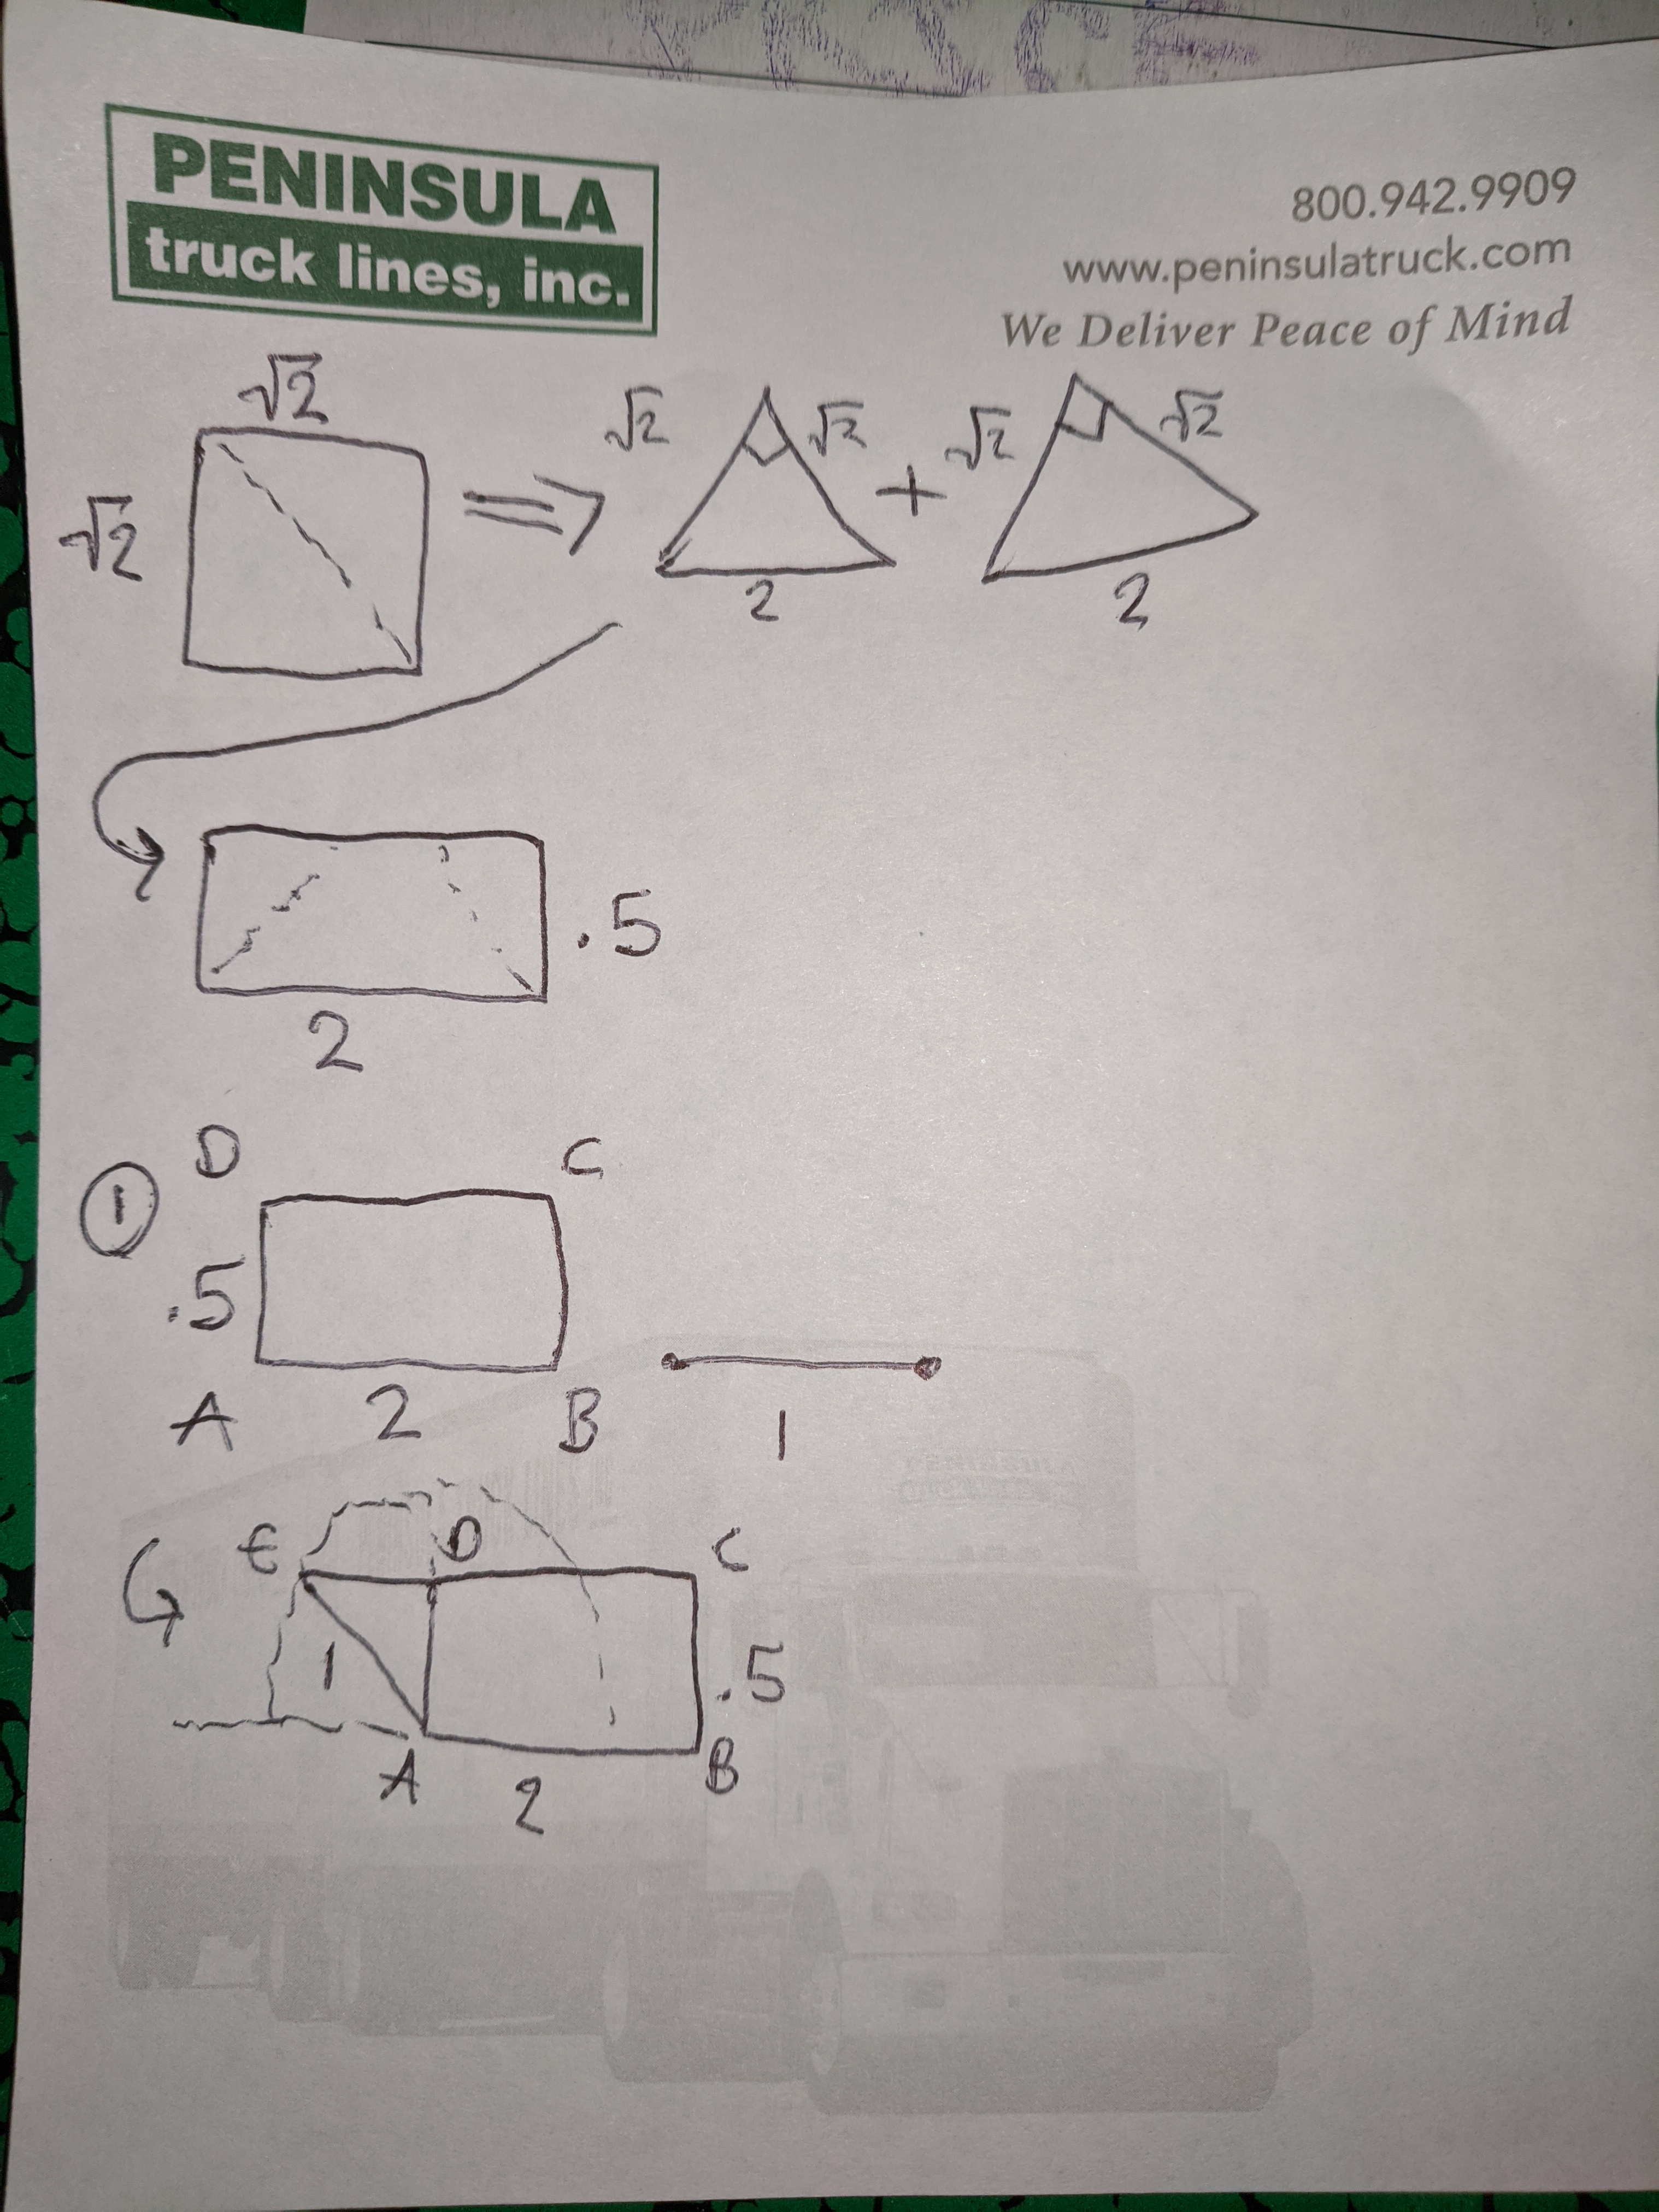
\includegraphics[width=10cm]{Ex 5.jpg}\\
\caption{Figure 1: Splitting the square into two trianlges and substep 1}\\
- This was a fairly easy and straightforward step. I took one of the .5 by 2 rectangles and put it into the algorithm to start to create a rectangle of base 1.\\
Substeps 2, 3, and 4:\\
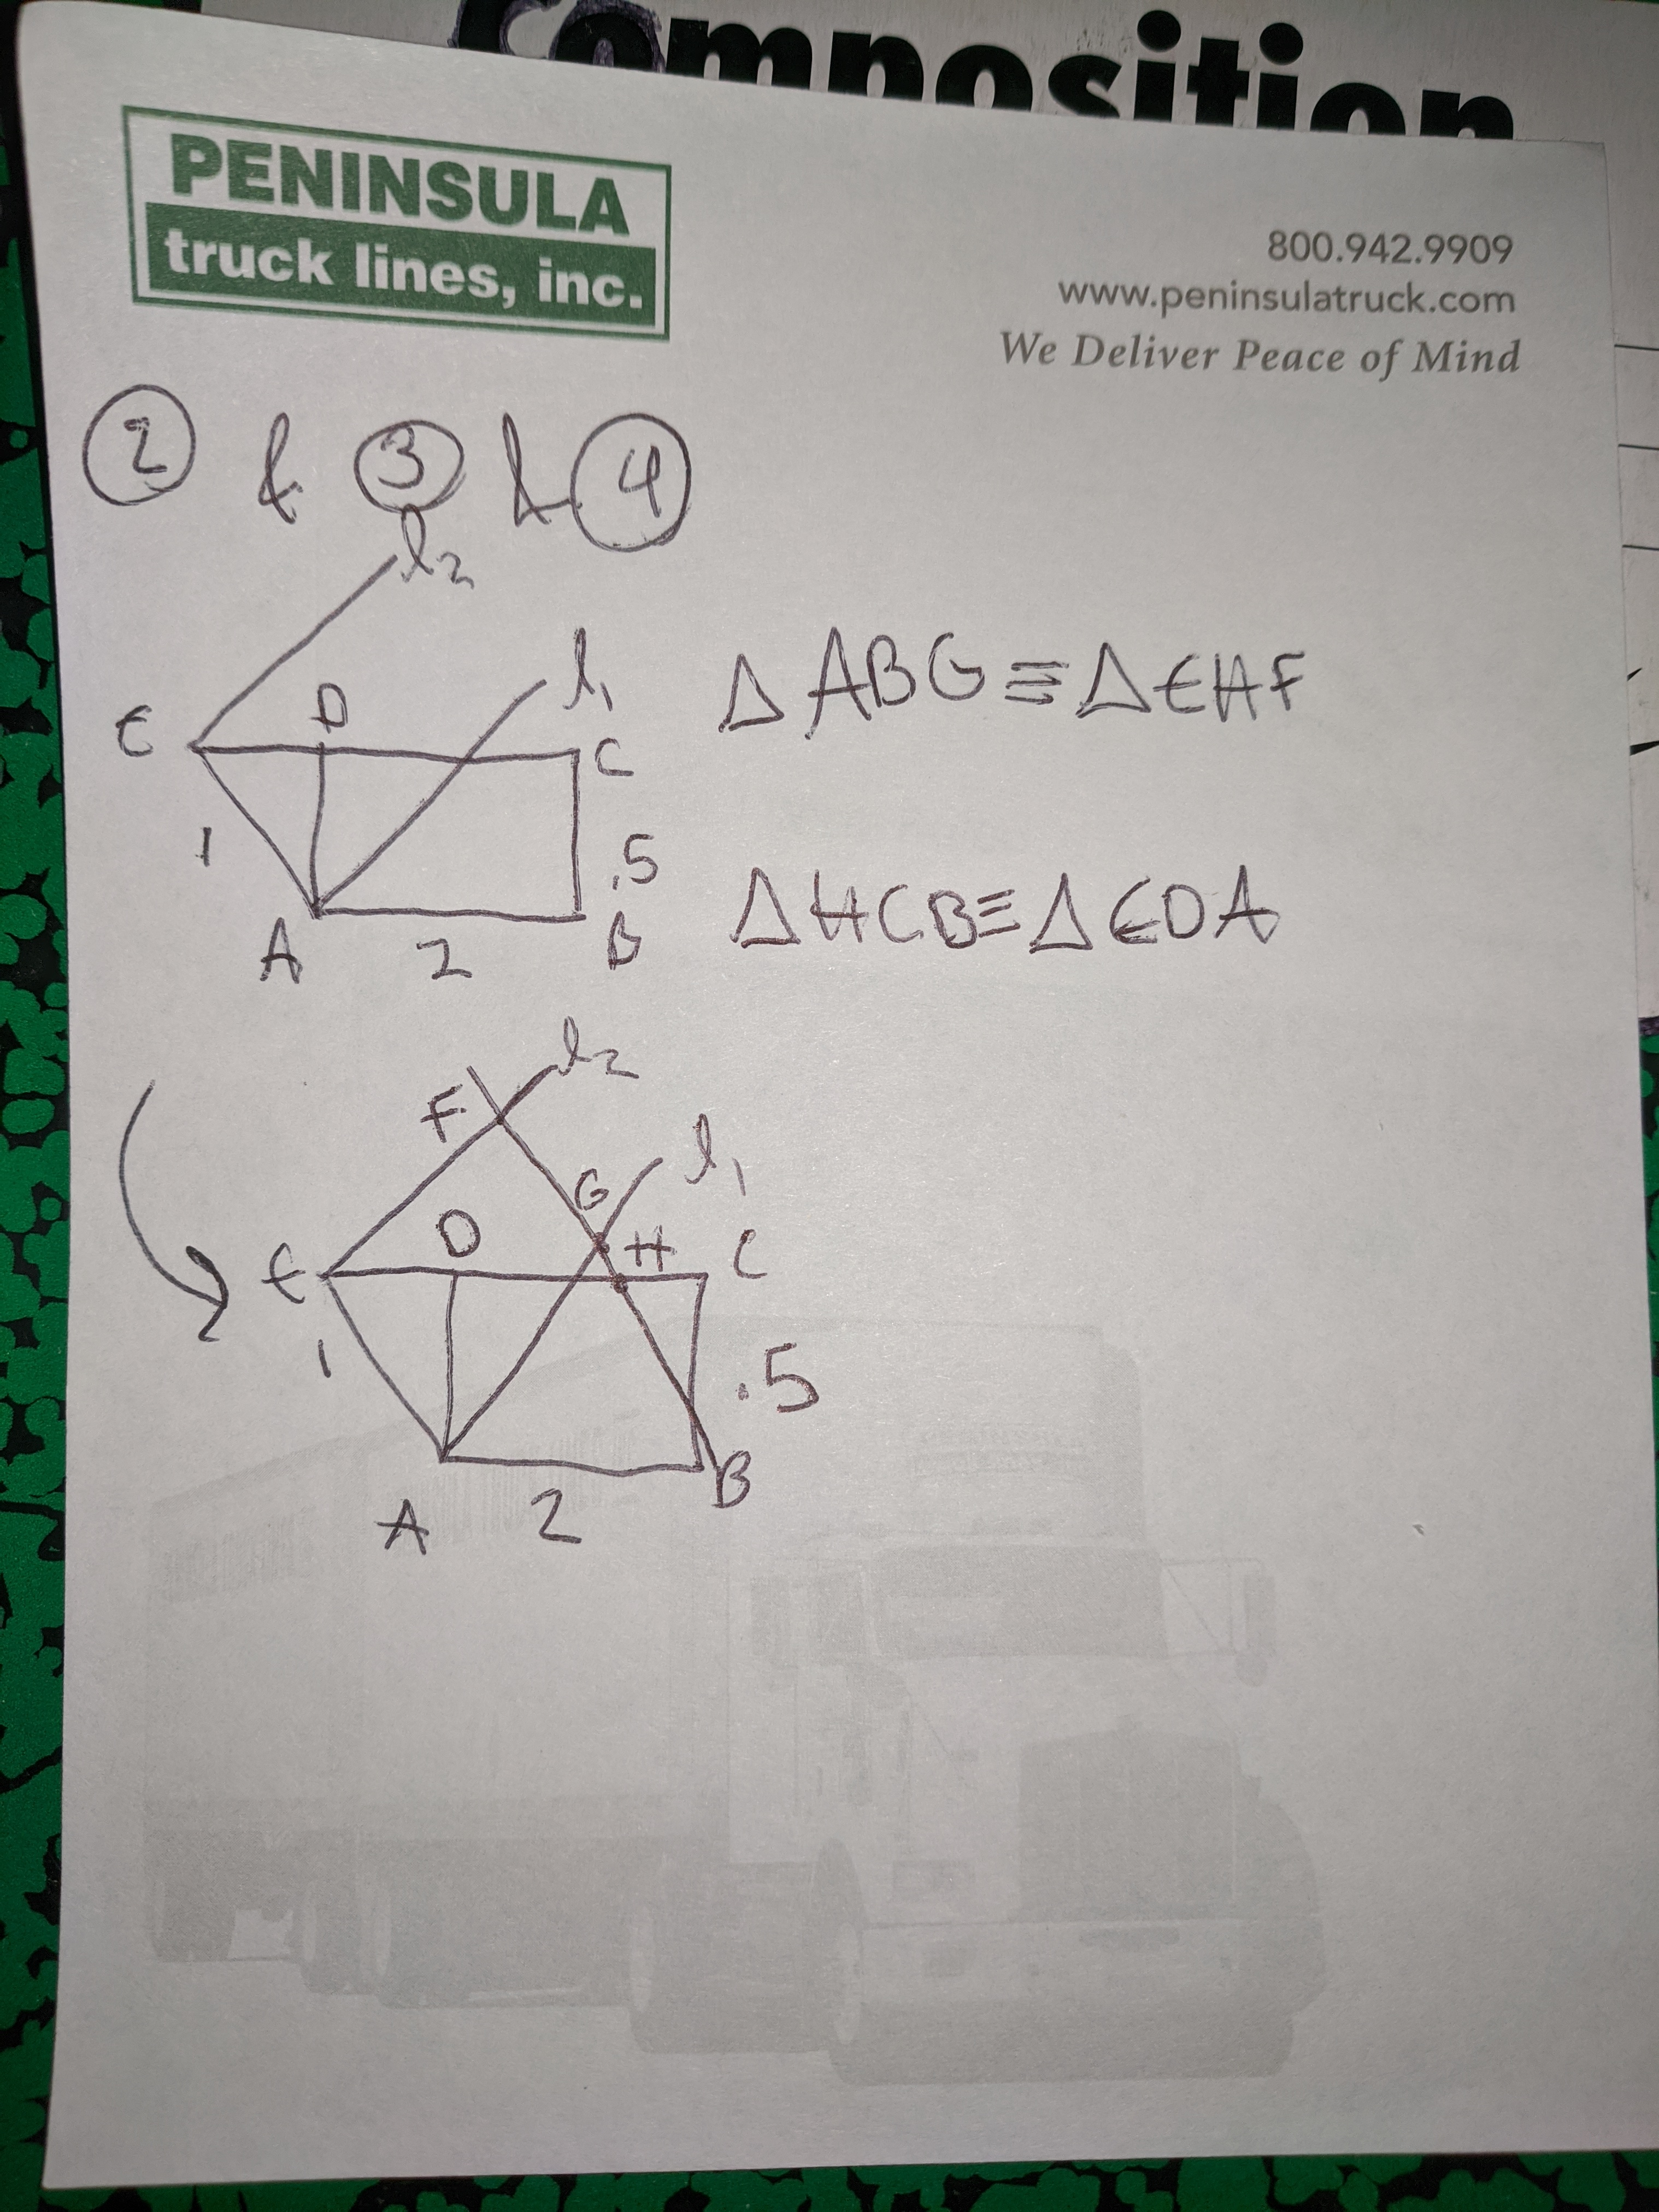
\includegraphics[width=10cm]{Ex 6.jpg}\\
\caption{Figure 2: Adding the length lines. Substeps 2, 3, and 4}\\
- As shown above, this is the same drawing, but with the two new added length lines and line FB. As written, triangles ABG and EHF are congruent as well as HCB and EDA. This is important later on to determine whether it worked correctly. This method produces two congruent rectangles which only works since various parts of both of them are congruent.\\
Substeps 5 and 6:\\



%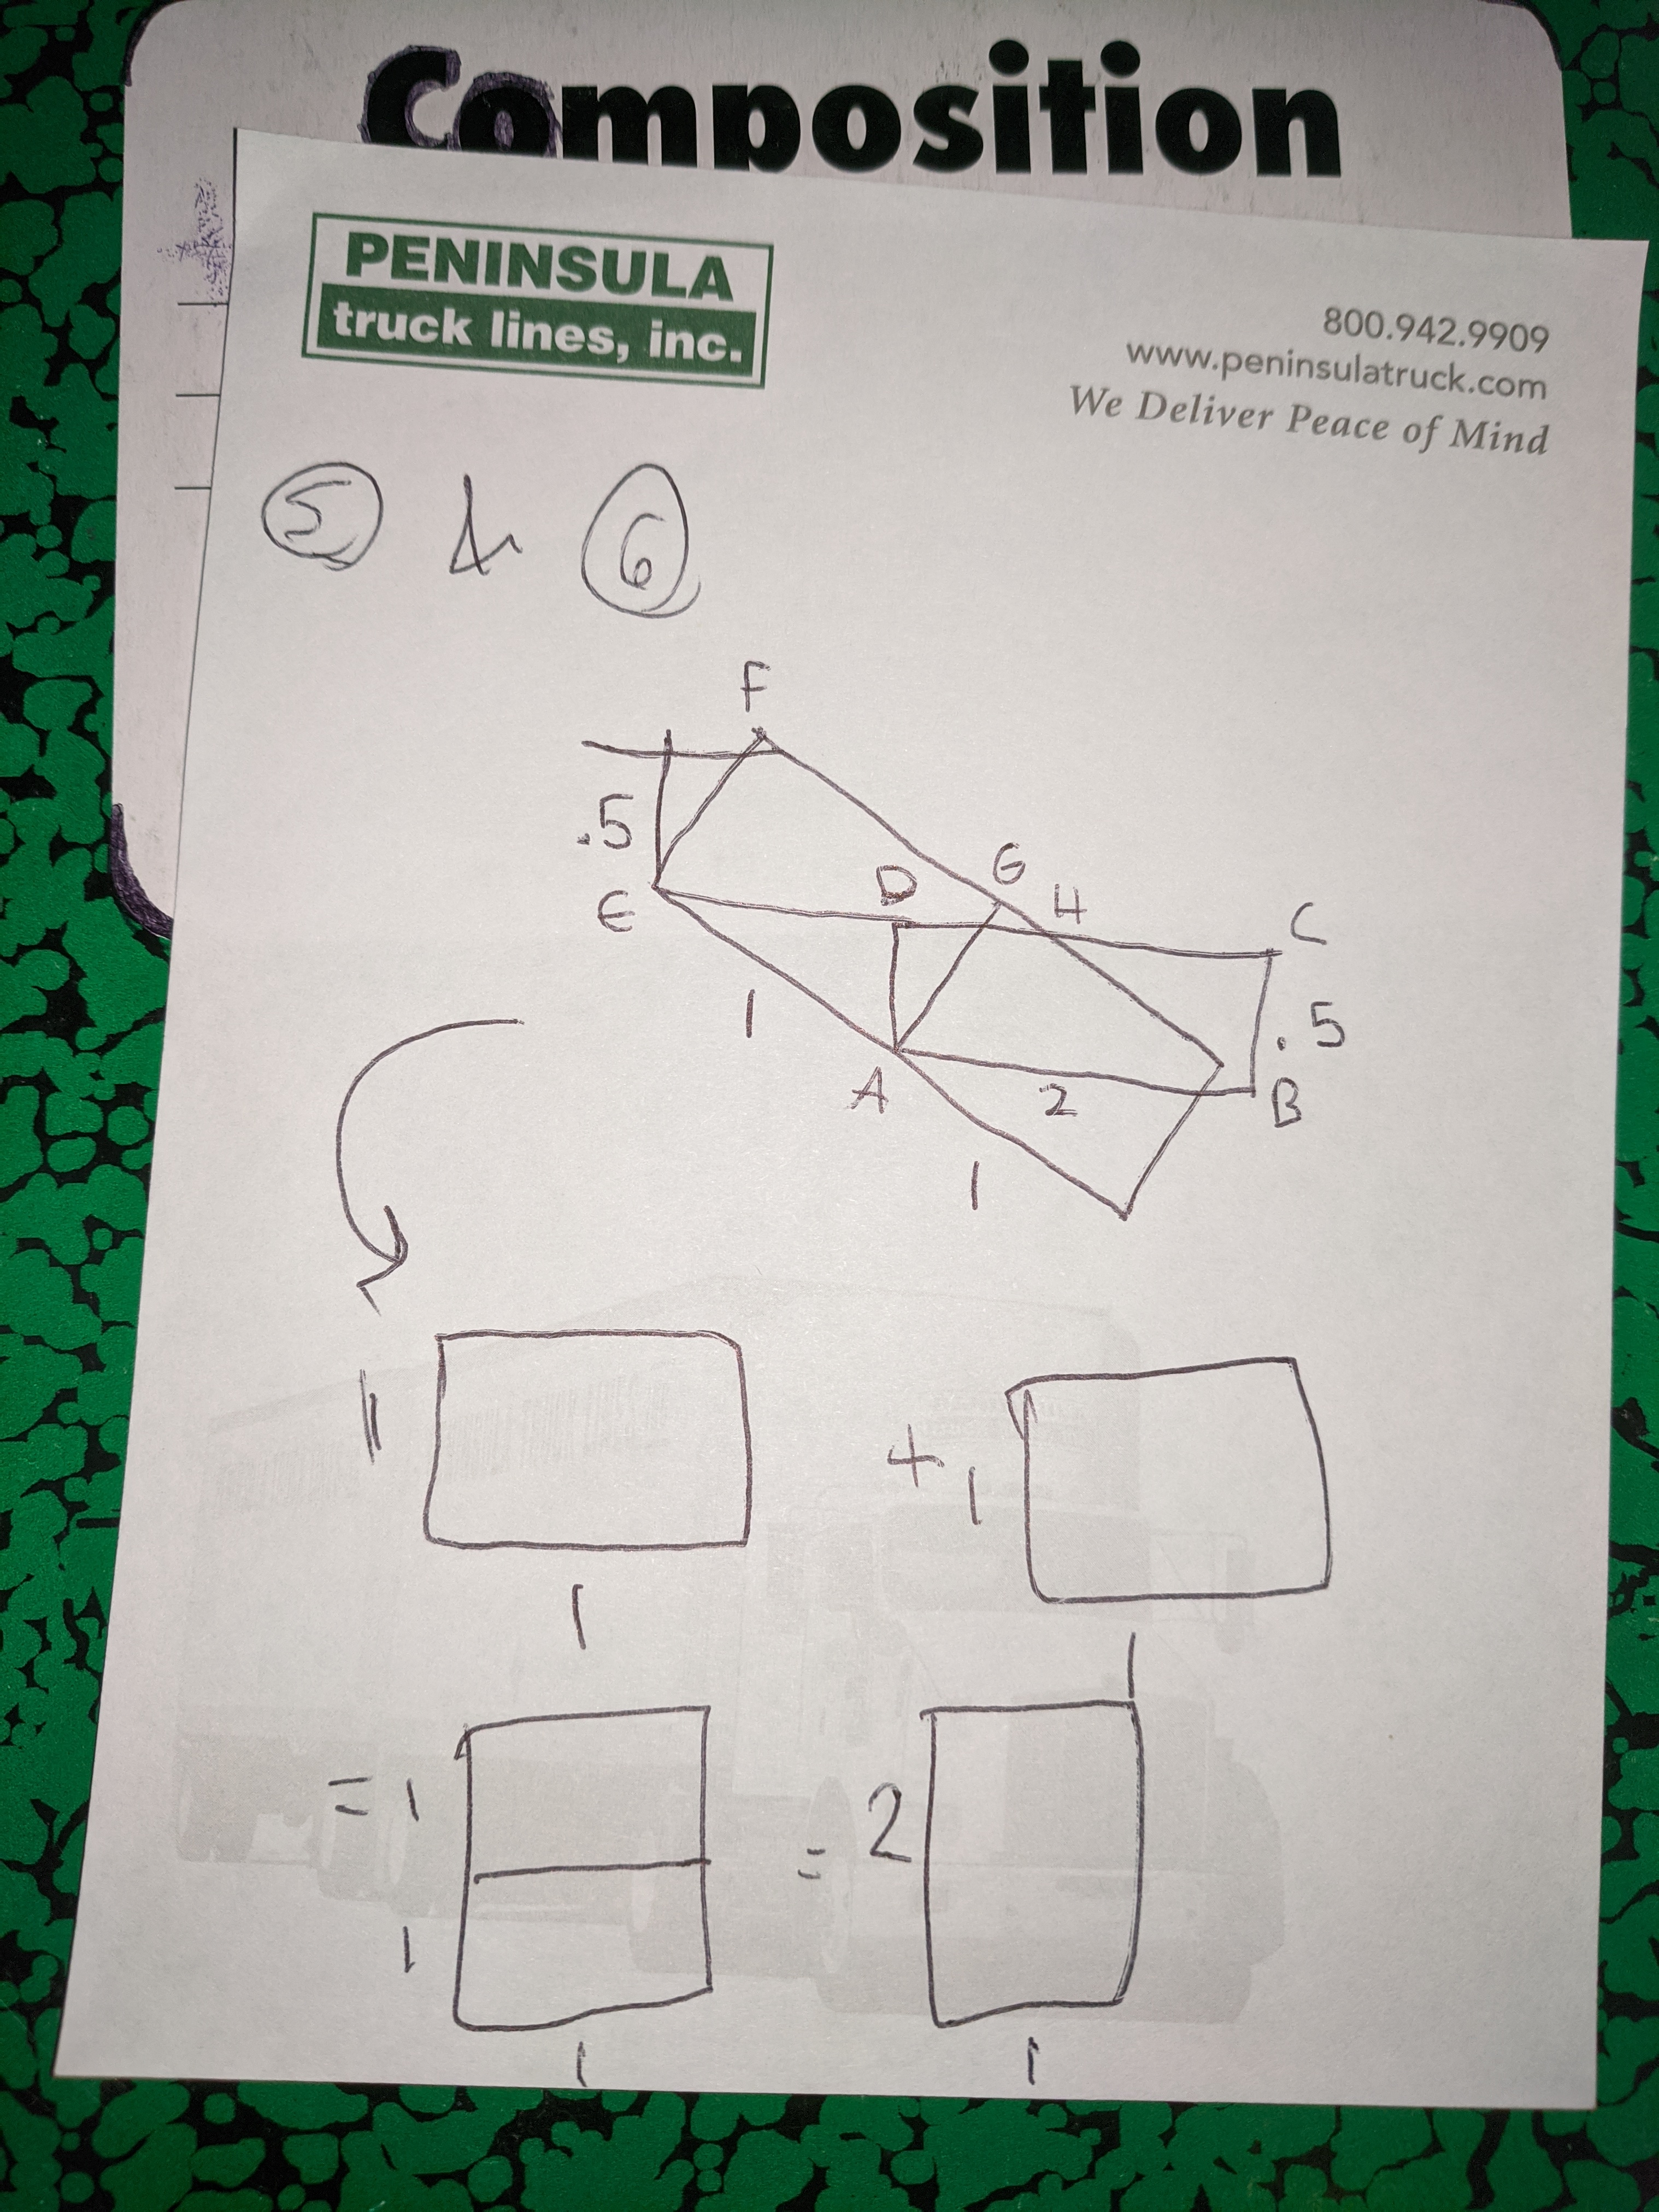
\includegraphics[width=10cm]{Ex 7.jpg}\\
%\caption{Figure 3: The final result. Substeps 5 and 6}\\

\begin{figure}[h]
    \centering
    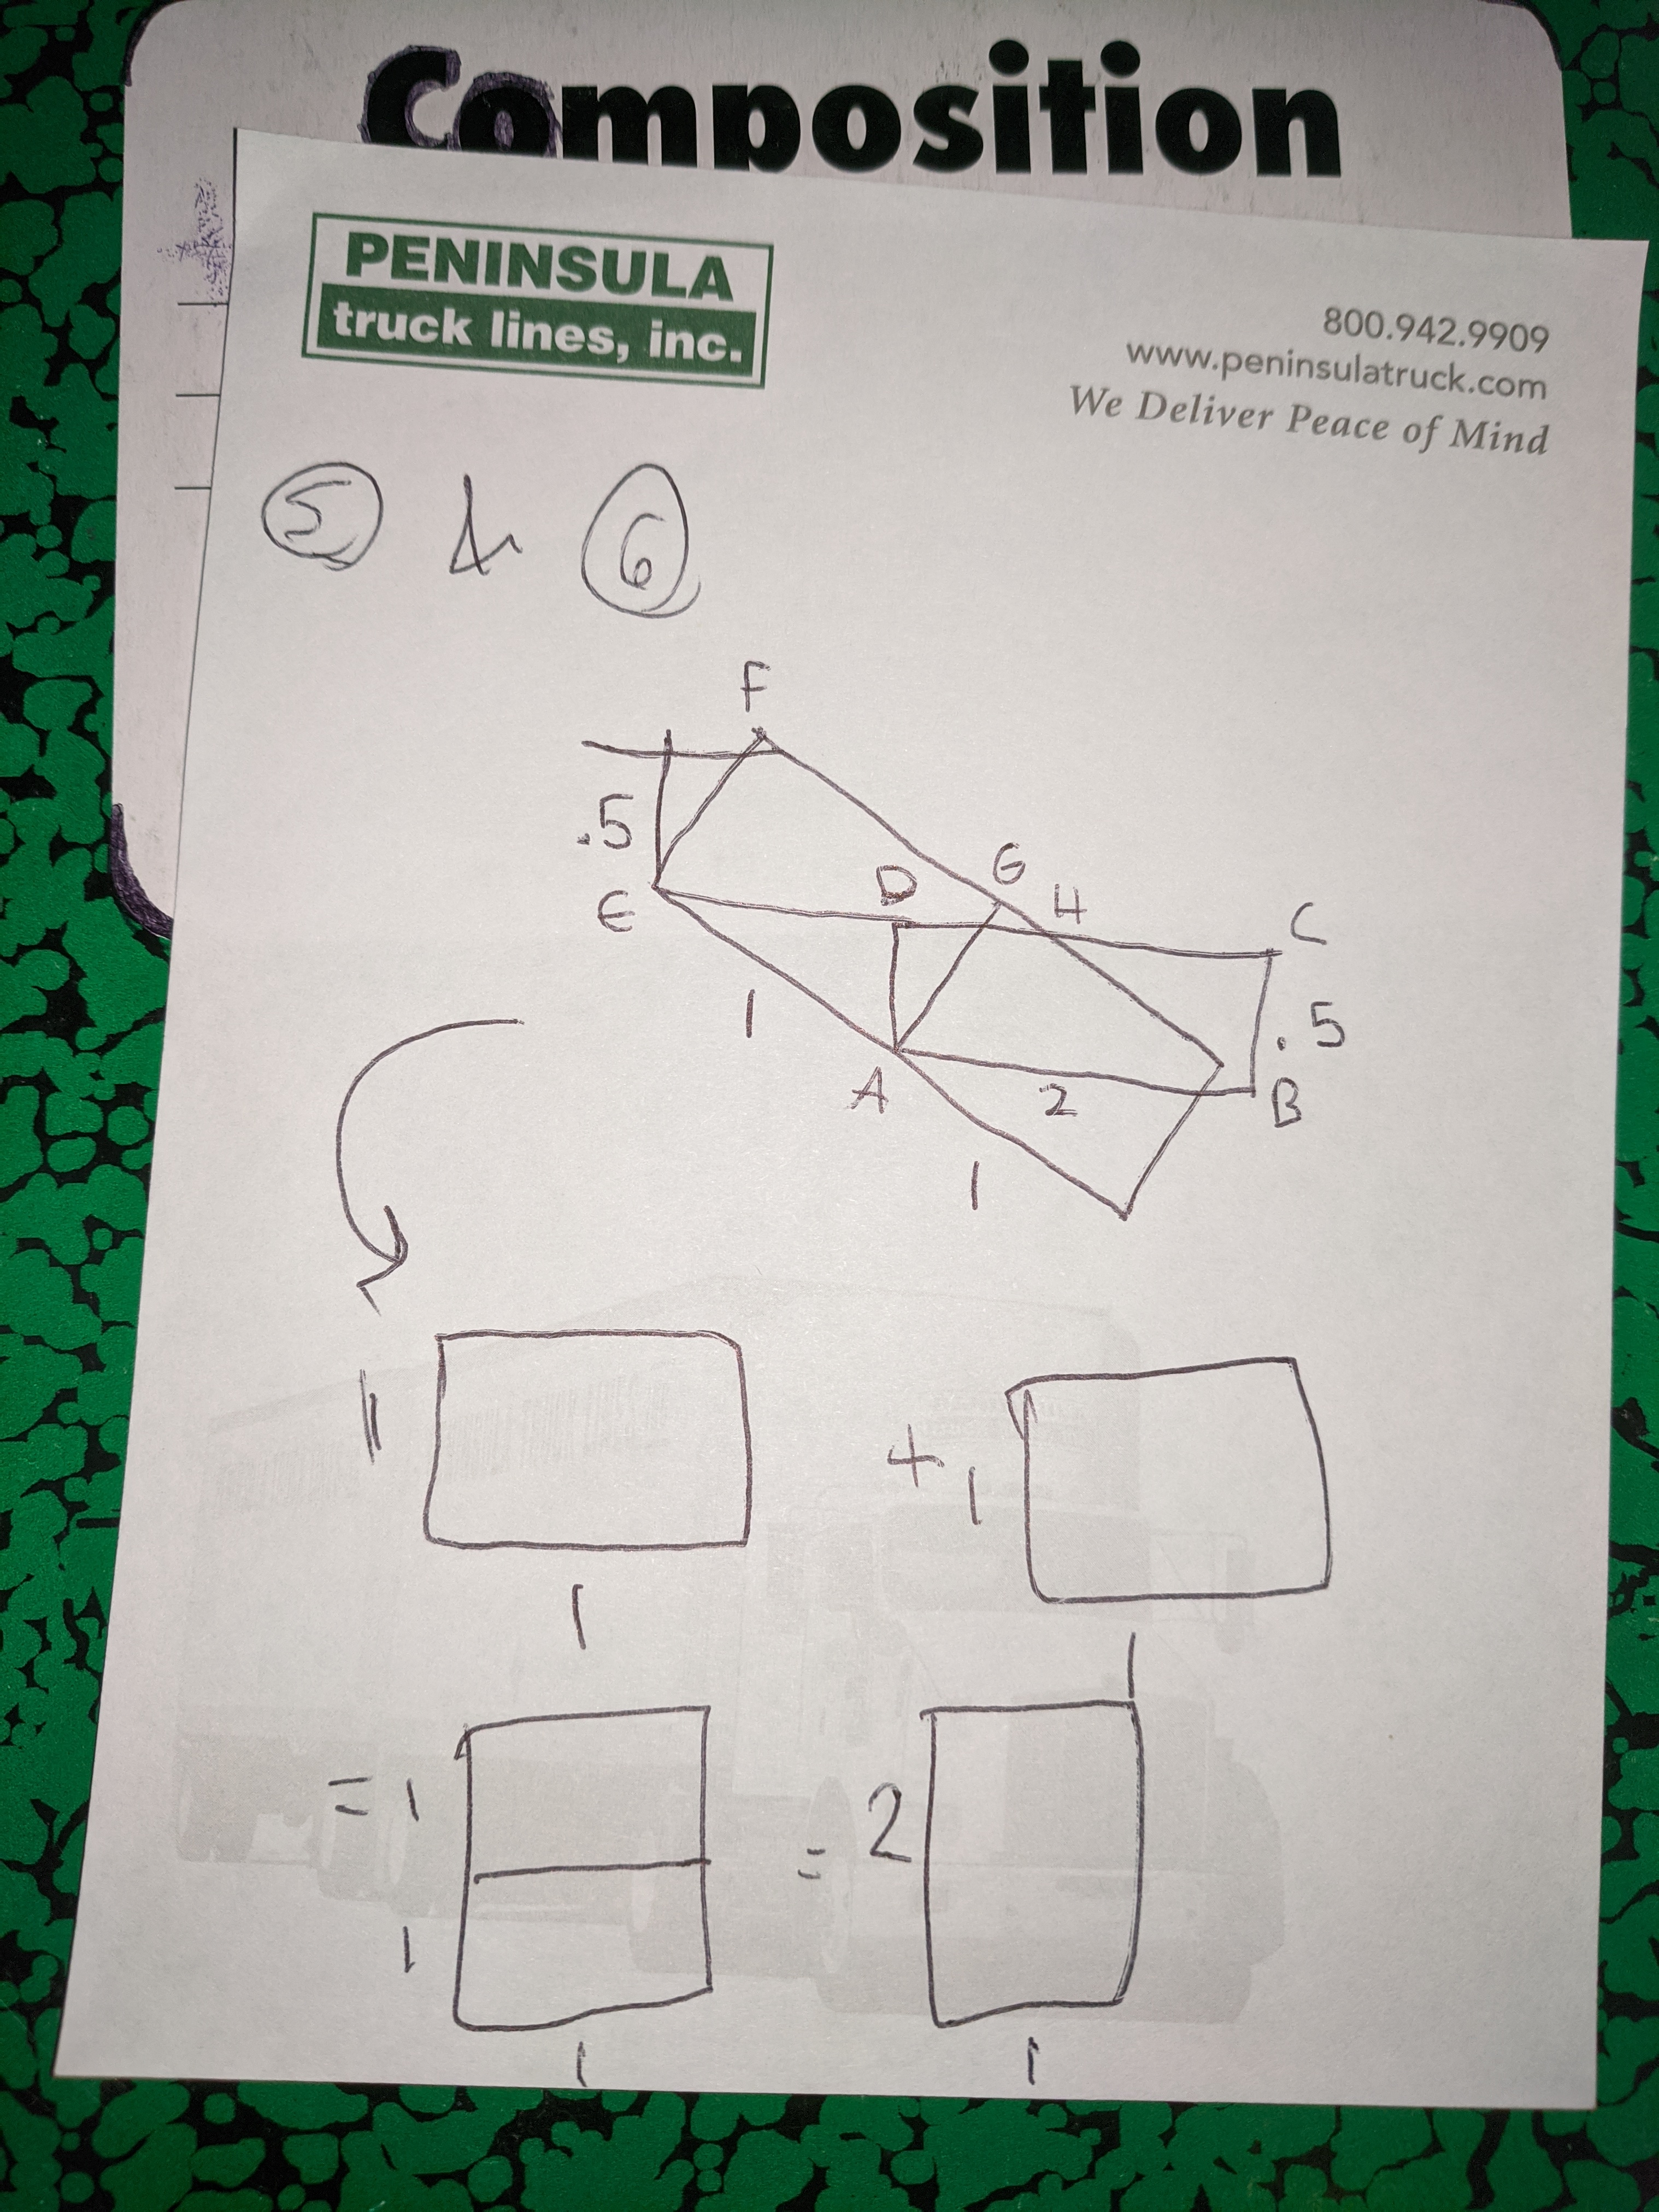
\includegraphics[width=10cm]{Ex 7.jpg}
    \caption{The final result. Substeps 5 and 6} 
    \label{fig_final_result}
\end{figure}

As Figure \ref{fig_final_result} shows the final result. The rectangle EFGA is what we are left with. If I am correct, it is 1 by 1 which also means it is a square. When this process is duplicated for the other triangle and we add both rectangles together, we are left with a 2 by 1 rectangle.\\
This process is backwards, but it gave me a great idea of what is going on. If this were done in reverse, we would be left with a $\sqrt{2}$ by $\sqrt{2}$ square. I hope it is okay that I did it backwards!\\

I also got confused with the /label and /ref commands. Could someone give me some advice on how to use those correctly?\\

% \label{rework_rectangle}
%
% \ref{rework_rectangle}
\\

\section*{Hannah's 3D Calculus Problem:}\\
- Hi, here is my understanding of a general way to find 3D angles using calculus. I wasn't given a specific problem, so I hope talking about it generally is okay. If I was given one, I'm sorry if I didn't see it! I would also like to add that 2/3 of my calculus classes so far were taught by an incredibly terrible teacher during my time at Pierce that didn't actually know how calculus worked. During Calc. III, my professor was actually removed from the course. No one got a good understanding of the content... Anything I am describing here was found out through online research. I am actually going to need a lot of help with this or anything else related to Calculus I or III!\\

Finding the angle between two 3D vectors is done by using a dot product. A dot product is found by multiplying corresponding elements of each vector together and adding the result.\\
For example, if vectors $a=\langle 2, 3, 4 \rangle$ and $b=\langle 6, 7, 8 \rangle$, then the dot product would be $(2)(6)+(3)(7)+(4)(8)=12+21+32=65$. This is also called $a \cdot b$.\\
$a \cdot b$ is used in a formula. This formula is $cos(\theta)=\frac{a \cdot b}{|a||b|}$. The next step is to find $|a|$ and $|b|$. This means to find the magnitude (length) of vectors $a$ and $b$. This is done by square each element in the vector, adding them together, and taking the square root of the total.\\
$|a|=\sqrt{2^2+3^2+4^2}=\sqrt{4+9+16}=\sqrt{29}$. This roughly equals 5.385.\\
$|b|=\sqrt{6^2+7^2+8^2}=\sqrt{36+49+64}=\sqrt{149}$. This roughly equals 12.207.\\
So far, the formula pieced together is $cos(\theta)=\frac{65}{(\sqrt{29})(\sqrt{149})}$.\\
The final step is to use the inverse of cosine to find $\theta$.\\
$cos(\theta)=\frac{65}{(\sqrt{29})(\sqrt{149})}$. The right side of this formula equals about 0.989.\\
$\theta = cos^{-1}(0.989)$. This means that $\theta$ equals about 8.506 degrees.\\

That is my example of how to find a 3D angle using calculus. Please let me know if I misinterpreted or missed anything I was supposed to do. Is this the right track? Please also let me know if I made any mistakes!\\
I used a short YouTube video for reference called "How to Find the Angle Between Two 3D Vectors" by Cowan Academy.\\
Thanks for reading my assignments!\\
P.S. I would like to record a video in the future for ease of explanation, but I am not sure how Zoom works beyond joining a class meeting. I didn't have much time this week to figure that out, but I could make more time in the future if you all think it would be easier or if there were any tips/tricks to share.\\

\section*{Addition to Previous Example, 8/16/20:}\\
In order for a more specific problem such as Ryan's example, I repeated this process for a 1 x 1 x 1 cube.\\
The vectors in question would be $a = \langle 1,1,1 \
\rangle$ and $b = \langle 1,0,0 \rangle$ because, when graphed out, would equal a border line of the cube and a line between two opposite corners.\\
In this case, $a \cdot b$ would equal $(1)(1)+(1)(0)+(1)(0)=1+0+0=1$.\\
$|a|=\sqrt{1^2+1^2+1^2}=\sqrt{1+1+1}=\sqrt{3}$ and $|b|\sqrt{1^2+0^2+0^2}=\sqrt{1+0+0}=\sqrt{1}=1$. This means that $|a||b|=\sqrt{3}$.\\
Therefore, the formula that we are left with is $cos(\theta)=\frac{1}{\sqrt{3}}$. The next step is to find the inverse of cos to find $\theta$.\\
$\theta= cos^{-1}(\sqrt{3})$ which equals $\theta=54.7356$ degrees. This is the angle between the two vectors.\\
I hope it was alright that I didn't choose to record a video for this assignment. Thank you Ruth for your instructions. I hope to record in the future, but when it comes to things like this, I tend to communicate them better over words that I can edit. Maybe next week I can write out a script for myself and record. Thanks for reading everyone!\\

\section*{Hannah's Next, Next Example:}\\
A plane in 3D space can be described as a sort of "floor" or "wall" that spans the entirety of 3D space on a certain equation. Two planes may intersect and create an angle between them.
The angles between two planes in 3D space are found using a similar formula used when finding the angles between vectors. This formula was found on https://onlinemschool.com/math/library/analytic$_$geometry/plane$_$angl/.\\
The formula states that if two planes are defined as\\
$A_1x+B_1y+C_1z+D_1=0$ and $A_2x+B_2y+C_2z+D_2=0$,\\
then $cos\alpha=\frac{|A_1*A_2+B_1*B_2+C_1*C_2|}{\sqrt{A_1^2+B_1^2+C_1^2}\sqrt{A_2^2+B_2^2+C_2^2}}$ (|| means absolute value here).\\
The two examples I created are $3x+4y+5z+6=0$ and $2x+7y+3z+5=0$. The formula, when plugged in, equals $cos\alpha = \frac{|3*2+4*7+5*3|}{\sqrt{9+16+25}\sqrt{4+49+9}}$.\\
This simplifies down to $cos\alhpa=\frac{49}{10*\sqrt{31}}$. Using $cos^{-1}$, $\alpha = 0.49479$.\\
As for the regular tetrahedron, I went to https://www.chegg.com/homework-help/questions-and-answers/plane-equation-x-y-b-z-c-1-b-c-0-together-positive-coordinate-planes-forms-tetrahedron-vol-q15557317 to find a formula. The formula is $\frac{x}{a}+\frac{y}{b}+\frac{z}{2}=1$ when $(a,b,c > 0)$.\\
The example that I used is $\frac{x}{1}+\frac{y}{1}+\frac{z}{1}=1$. This means that point $A=(1,0,0)$, point $B=(0,1,0)$, and point $C=(0,0,1)$. The other sides are the axes, as shown on the website that I have linked.\\
The formula becomes $x+y+z=1$ when simplified. We are going to compare this to the side plane of axis $x$. The equation of this plane is $y=0$.\\
When plugged into the previous formula, we get $cos\alpha=\frac{|1*0+1*1+1*0|}{\sqrt{1^2+1^2+1^2}\sqrt{0^2+1^2+0^2}}$. This simplifies into $cos\alpha=\frac{1}{\sqrt{3}}$.\\
Using inverse $cos$, $\alpha=0.95531$. This is the angle between the planes of a regular tetrahedron.\\
Thanks for reading! :)\\

\section*{Hannah's Regular Tetrahedron:}\\
- I started out by drawing a tetrahedron inside of a cube that looks like the one pictured in this link:\\
http://gogeometry.com/solid/cube$_$tetrahedron.htm\\
I followed your advice and turned the cube into the axes that I would base my tetrahedron off of so it was regular this time around. I placed the axes such that the corners of the cube are at the coordinates of (0,0,0), (1,0,0), (0,1,0), (0,0,1), (1,1,0), (0,1,1), (1,0,1), and (1,1,1). Let me know if that doesn't make much sense, and I will try to explain further. I recognize it does sound a little confusing.\\
The four points of the tetrahedron are at the coordinates (1,0,0), (0,0,1), (0,1,0), and (1,1,1). The equations for two planes of this regular tetrahedron are going to be found using three of the points that both planes touch. I found this technique at this link:\\
https://brilliant.org/wiki/3d-coordinate-geometry-equation-of-a-plane/#:~:text=If%20we%20know%20the%20normal,of%20the%20plane%20is%20established.&text=a%20(%20x%20%E2%88%92%20x%201%20),%E2%88%92%20z%201%20)%20%3D%200.\\
(I am unsure how to fix that link, sorry!)\\
For the first plane, I will use the points A = (1,0,0), B = (0,0,1), and C = (1,1,1).\\
Using the basic formula $ax+by+cz+d=0$, we will input each digit of the coordinate into the formula separately and then put all three formulas together.\\
This results in:\\
$1a+0b+0c+d=0$\\
$0a+0b+1c+d=0$\\
$1a+1b+1c+d=0$\\
which reduce to\\
$a+d=0$\\
$c+d=0$\\
$a+b+c+d=0$.\\
The next step is to set these equations equal to each other to find $b,c,$ and $d$ in terms of $a$. The results of this are $b=-a$, $c=a$, and $d=-a$. Substituting these variables into the equation, we get $ax-ay+az-a=0$ which equals $x-y+z-1=0$.\\
Repeating this process with another plane, we will use the points A = (0,1,0), B = (0,0,1), and C = (1,1,1). Inputting them into the formula equals\\
$0a+1b+0c+d=0$\\
$0a+0b+1c+d=0$\\
$1a+1b+1c+d=0$\\
which reduces to\\
$b+d=0$\\
$c+d=0$\\
$a+b+c+d=0$.\\
Setting these three equations equal to each other results in $b=-a$, $c=-a$, and $d=a$. The new equation is $ax-ay-az+a=0$ which equals $x-y-z+1=0$.\\
The next step is to repeat my process from my last assignment by using $cos\alpha=\frac{|A_1*A_2+B_1*B_2+C_1*C_2|}{\sqrt{A_1^2+B_1^2+C_1^2}\sqrt{A_2^2+B_2^2+C_2^2}}$. Plugging in the variables here creates $cos\alpha=\frac{|(1*1)+(-1*-1)+(1*-1)|}{\sqrt{(1)^2+(-1)^2+(1)^2}\sqrt{(1)^2+(-1)^2+(-1)^2}}$ which reduces to $cos\alpha=\frac{1}{3}$. Using $cos^{-1}$, $\alpha=1.23095$.\\
Thanks for reading! Please let me know if there are any errors. The 0's and 1's blurred together. I did triple check my math though!


\end{document}
